\section{Design architetturale}

% questa sezione deve essere sufficiente per uno sviluppatore per giungere ad un sistema che è organizzato come il nostro

% (architettura complessiva, descrizione di pattern architetturali usati, componenti del sistema distribuito, scelte tecnologiche cruciali ai fini architetturali -- corredato da pochi ma efficaci diagrammi)

% Ricordate che una scelta architetturale può ritenersi giustificata o meno solo a fronte dei requirement che avete indicato; viceversa, ogni requirement "critico" dovrebbe influenzare qualcuna della scelte architetturali effettuate e descritte.
% L'architettura deve spiegare quali sono i sotto-componenti del sistema (da 5 a 15, diciamo), ognuno cosa fa, chi parla con chi e per dirsi cosa -- i diagrammi aiutano, ma poi la prosa deve chiaramente indicare questi aspetti.

Il gruppo ha scelto di lasciare la libreria non vincolata da dipendenze esterne oltre alla scelta del linguaggio Scala, dettata dai requisiti.
%
Non sono infatti state utilizzate librerie esterne se non quelle per il testing automatizzato.

Nel descrivere il design architetturale nelle sotto-sezioni seguenti, viene prima effettuata un'analisi del dominio, successivamente si passa alla descrizione dei pattern architetturali utilizzati.

% ---------------------------------------------------

\subsection{Analisi del dominio}

Il risultato dell'analisi del dominio dei giochi da tavolo è rappresentato in Figura \ref{fig:domain_analysis}.
%
L'analisi ha evidenziato la presenza costante di una divisione in \textbf{aspetti intensionali}, ovvero fissati indipendentemente da una specifica partita, ed \textbf{aspetti estensionali}, che catturano dettagli legati al gioco durante il suo svolgimento.

\begin{figure}
  \centering
  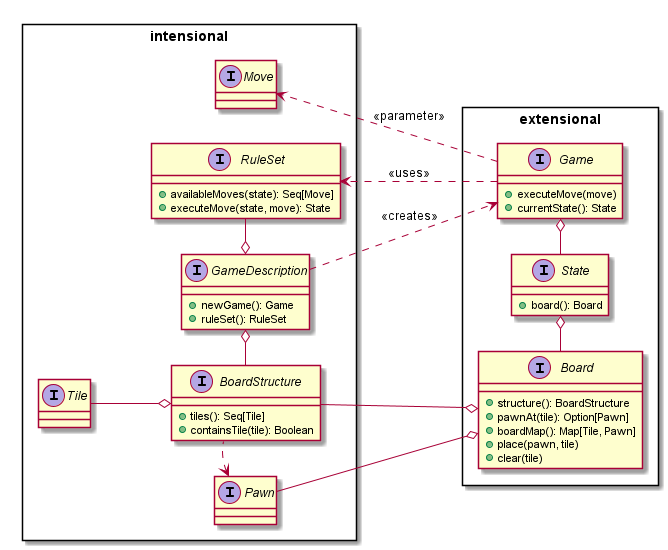
\includegraphics[width=\linewidth]{images/uml/domain_analysis.png}
  \caption{Diagramma delle classi rappresentante il risultato dell'analisi del modello del dominio}
  \label{fig:domain_analysis}
\end{figure}

\paragraph{Aspetti intensionali}
I concetti intensionali sono visibili nella porzione di sinistra del diagramma in Figura \ref{fig:domain_analysis}.

Il nucleo di questo insieme di entità è costituito dalla \texttt{GameDescription}, che rappresenta la definizione principale di un gioco e viene utilizzata per crearne nuove istanze.
%
Ad ogni \texttt{GameDescription} è associato un \texttt{RuleSet}, che contiene la logica per la generazione e l'esecuzione delle mosse disponibili per un dato stato della partita, e una \texttt{BoardStructure} contenente la disposizione dei \texttt{Tile} che costituiscono il tabellone di gioco e il tipo di \texttt{Pawn} che possono ospitare.

Infine, fanno parte degli aspetti intensionali anche le \texttt{Move}, che racchiudono tutte le informazioni necessarie al \texttt{RuleSet} per l'esecuzione della mossa stessa.

\paragraph{Aspetti estensionali}
A livello estensionale, le entità individuate sono collocate nella metà di destra del diagramma in Figura \ref{fig:domain_analysis}.

La radice di questo gruppo di entità è il \texttt{Game}, ovvero la rappresentazione di una istanza attiva di partita.
%
Ad esso è affidato il compito di mantenere consistente lo \texttt{State} della partita a fronte dell'esecuzione delle \texttt{Move} e utilizza quindi il \texttt{RuleSet} per garantire questa proprietà.

Uno \texttt{State} contiene tutte le informazioni necessarie a definire un istante legale del proseguimento della partita, comprendente di stato della \texttt{Board}, giocatori attivi, turni, ecc.
%
Non tutti questi aspetti sono condivisi da tutti i giochi da tavolo, e sono perciò omessi nel diagramma ad eccezione della \texttt{Board}, che è sempre presente.

Infine, la \texttt{Board} è l'entità che definisce e manovra la disposizione dei \texttt{Pawn} sui \texttt{Tile} definiti dalla sua \texttt{BoardStructure}.
%
La \texttt{Board} deve anche imporre il vincolo di avere al più un \texttt{Pawn} su ogni \texttt{Tile}.

\paragraph{Aspetti comuni dei giochi da tavolo}
%
Si analizzano ora gli aspetti trasversali a tutti i giochi da tavolo.
%
\subparagraph{Turni e Giocatori}
%
I giochi da tavolo sono quasi sempre suddivisi in turni che scandiscono il flusso di una partita; un turno solitamente identifica una serie di azioni che possono essere svolte prima della sua terminazione.
%
Ogni gioco, inoltre, ha un numero fisso di giocatori che prendono parte ad una partita (un gioco con zero giocatori è da intendersi come un simulatore e non più un gioco).
%
Il sistema dei turni e quello dei giocatori sono quasi sempre fortemente legati tra loro e in molti casi i concetti di turno e di giocatore sono sovrapposti tra loro ed è possibile utilizzare entrambi senza distizione.
%
Non si faranno, quindi, distinzioni tra turno e giocatore se non nei casi in cui questi risultini diversi tra loro.
%
\subparagraph{Condizioni di terminazione}
%
Queste identificano l'insieme di condizioni necessarie e sufficienti affinchè una partita termini.
%
Le partite possono terminare solitamente in due modi:
\begin{itemize}
  \item vittoria di un giocatore: caso in cui un giocatore ha raggiunto i requisisti per essere dichiarato vincitore.
  \item pareggio: caso in cui nessun giocatore è dichiarato vincitore;
\end{itemize}
% Turni
% Giocatori
% Condizioni di terminazione

% ---------------------------------------------------

\subsection{Pattern architetturali}
% descrizione di pattern architetturali usati, MVC
Data la natura del progetto è risultato necessario fornire delle astrazioni ben consolidate.
%
In particolare, per applicazioni che si basano sull'interazione utente, il pattern \textbf{MVC} è uno dei più noti e flessibili.

% MVC
%Perché, analisi del problema
La separazione delle responsabilità fra i vari componenti è uno dei motivi principali per cui è stato scelto questo pattern: è infatti possibile per un utente della libreria descrivere totalmente un gioco senza fare alcun riferimento alla sua rappresentazione, e solo successivamente collegare ad esso interazione e visualizzazione.
%
Questo è di particolare importanza in una libreria come SBAGS in quanto diversi tipi di interfaccia potrebbero essere necessari per diversi tipi di giochi, e correlare presentazione a modello lo renderebbe più complesso e dispendioso.

Un'ulteriore motivazione risiede nell'abilitare la possibilità di fornire più modalità di visualizzazione del gioco e di interpretazione dell'input utente che possano essere direttamente utilizzabili dagli utenti della libreria.

% ---------------------------------------------------

\subsection{Architettura complessiva}
%In quale modo
% 0. architettura complessiva, -- model, controller & subcontoller, view & subView:
L'interpretazione del pattern MVC adottata in questo progetto è basata su gerarchie di controller e di view: ogni fase dell'applicazione - e.g. menu, partita in corso - ha una sua coppia di view e controller che gestiscono la specifica situazione.

\subsubsection{Avanzamento delle fasi dell'applicazione}
% 1. class diagram
\begin{figure}
  \centering
  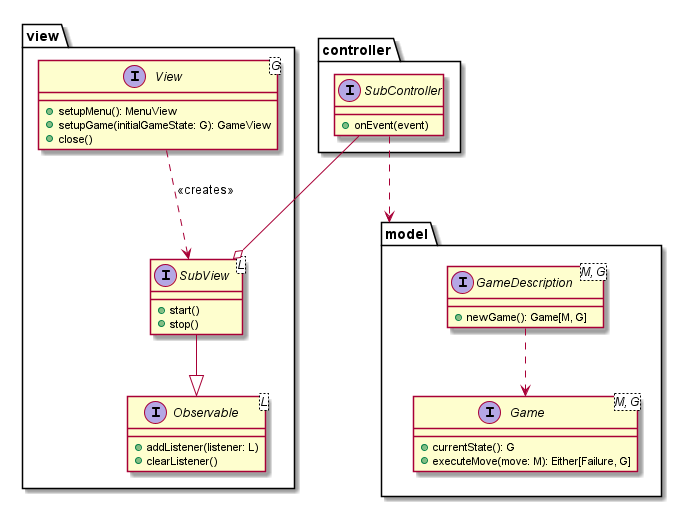
\includegraphics[width=\linewidth]{images/uml/main_class_diagram.png}
  \caption{Diagramma rappresentante le principali interfacce di model, view e controller}
  \label{fig:main_class_diagram}
\end{figure}
Come mostrato in figura \ref{fig:main_class_diagram} è possibile, tramite la \texttt{View} principale, generare le \texttt{SubView} a cui associare i vari \texttt{SubContoller}.
I \texttt{SubContoller} incapsulano la logica per passare da una \texttt{SubView} all'altra e di conseguenza da una fase dell'applicazione ad un'altra.

\subsubsection{Interazioni MVC}
% 2. interazione C - V con registrazione/deregistrazione dei listener
In fase di definizione, ogni \texttt{SubView} specifica il proprio tipo di listener (\texttt{SubContoller}).
%
I listener, dopo essere stati aggiunti, vengono notificati seguendo il pattern \textbf{Observer}, in base agli eventi che accadono alla relativa \texttt{SubView}.
% 3. interazione in game -> scambio di messaggi tra GameController e GameView (+ model) -> sequence diagram
Come mostrato in figura \ref{fig:gui_sequence}, alcuni \texttt{SubContoller}, in particolare quelli che gestiscono le interazioni di gioco sono in grado di gestire l'interazione con il \texttt{model}: date delle combinazioni di eventi valide per il gioco specifico, il \texttt{SubContoller} è in grado di far avanzare lo stato della partita facendo eseguire una \textit{move} al model.
%
Il model può rispondere con un nuovo stato o con un errore, in entrambi i casi il \texttt{SubContoller} inoltra il messaggio alla \texttt{SubView} per mostrare a schermo l'avanzamento o l'errore.
%% sequence diagram
\begin{figure}
  \centering
  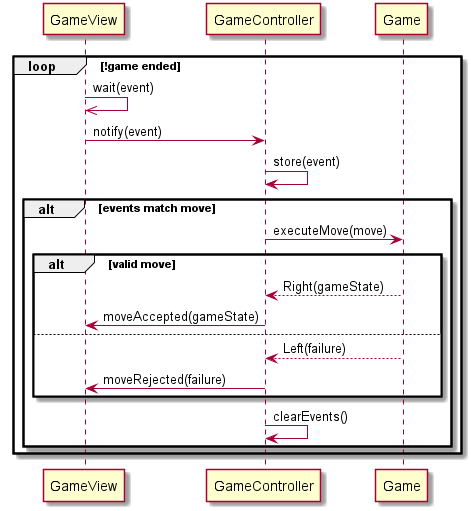
\includegraphics[width=\linewidth]{images/uml/gui_sequence.png}
  \caption{Diagramma di sequenza rappresentante le interazioni in un game tra model, view e controller}
  \label{fig:gui_sequence}
\end{figure}